% Wyrd III tutorial. Build: make (Tectonic). Screenshots: images/, command output: transcripts/;
% both are regenerated from real runs by shots/make_shots.py.
\documentclass[11pt]{article}
\usepackage[OT1]{fontenc}
\usepackage{mathptmx}
\usepackage[scaled=.90]{helvet}
\usepackage{courier}
\usepackage[letterpaper,margin=1.1in,top=1.0in,bottom=1.0in]{geometry}
\usepackage{graphicx,xcolor,fancyhdr,titlesec,caption,enumitem,fancyvrb,listings,float,url}
\usepackage[colorlinks=true,linkcolor=blue!60!black,urlcolor=blue!60!black]{hyperref}

\definecolor{banner}{HTML}{1F5FBF}
\definecolor{codebg}{HTML}{F4F4F4}
\definecolor{cmt}{HTML}{2E7D32}

\titleformat{\section}{\sffamily\Large\bfseries}{\thesection}{0.8em}{}
\titleformat{\subsection}{\sffamily\large\bfseries}{\thesubsection}{0.8em}{}
\titlespacing*{\section}{0pt}{16pt}{8pt}
\titlespacing*{\subsection}{0pt}{12pt}{5pt}

\pagestyle{fancy}
\fancyhf{}
\lhead{\scriptsize\textsc{Wyrd III Tutorial: Projects, VTR, Simulation and Midgard III}}
\rhead{\scriptsize\textit{For Wyrd III 0.1}}
\lfoot{\small Yggdrasil III}
\rfoot{\small\thepage}
\renewcommand{\headrulewidth}{0.3pt}
\renewcommand{\footrulewidth}{0pt}

\setlength{\parindent}{0pt}
\setlength{\parskip}{6pt}
\captionsetup{font=small,labelfont=bf,labelsep=period}
\setlist[enumerate]{leftmargin=2.2em,itemsep=4pt,topsep=2pt}
\setlist[itemize]{itemsep=2pt,topsep=2pt}

% UI labels and commands
\newcommand{\ui}[1]{\textsf{#1}}
\newcommand{\menu}[1]{\textsf{#1}}
\newcommand{\cmd}[1]{\texttt{#1}}
\newcommand{\gt}{\,\textsf{>}\,}

% Pasted real output (transcripts/*.txt are written by shots/make_shots.py)
\DefineVerbatimEnvironment{Out}{Verbatim}{fontsize=\footnotesize,frame=single,rulecolor=\color{gray},
  framesep=3pt,baselinestretch=0.95}
\newcommand{\transcript}[1]{{\VerbatimInput[fontsize=\footnotesize,frame=single,rulecolor=\color{gray},
  framesep=3pt]{transcripts/#1.txt}}}
\newcommand{\widetranscript}[1]{{\VerbatimInput[fontsize=\scriptsize,frame=single,rulecolor=\color{gray},
  framesep=3pt]{transcripts/#1.txt}}}

\lstset{basicstyle=\ttfamily\footnotesize,backgroundcolor=\color{codebg},frame=single,
  rulecolor=\color{gray},keywordstyle=\bfseries,commentstyle=\color{cmt}\itshape,columns=fullflexible,
  keepspaces=true,showstringspaces=false,breaklines=true,xleftmargin=0pt}
\lstdefinelanguage{Verilog}{morekeywords={module,endmodule,input,output,wire,reg,always,posedge,
  if,else,begin,end,assign,parameter},sensitive=true,morecomment=[l]{//},morecomment=[s]{/*}{*/}}
\lstdefinelanguage{TOMLx}{morekeywords={},morecomment=[l]{\#},morestring=[b]"}

\newcommand{\shot}[3][1.0]{\begin{figure}[H]\centering
  \includegraphics[width=#1\linewidth]{images/#2.png}\caption{#3}\label{fig:#2}\end{figure}}

\newcommand{\note}[1]{\par\smallskip\noindent\fbox{\parbox{0.94\linewidth}{\small\textbf{Note.} #1}}\par\smallskip}

\begin{document}

\begin{center}
{\sffamily\LARGE Wyrd III Tutorial\\[2pt] Projects, VTR, Simulation and Midgard III}
\end{center}
\vspace{2pt}
\noindent\colorbox{banner}{\parbox{\dimexpr\linewidth-2\fboxsep}{\color{white}\sffamily\itshape\small For Wyrd III 0.1\quad(Yggdrasil III suite)\hfill October 2026}}

\section{Introduction}

This tutorial shows how to use Wyrd III, the experiment runner and workbench around the Odin III
synthesis front end. You will build a small project of your own from an empty folder, run it through
Odin III and VTR, read the results, look at it in the graphical interface, simulate it cycle by cycle,
and then use the ready-made content that comes with Wyrd III: the sample project and the Midgard III game.

Doing this tutorial, the reader will learn about:
\begin{itemize}
\item Installing Wyrd III and describing your machine to it
\item Writing a Verilog design and a \cmd{wyrd.toml} project file
\item Running the design through Odin III and VPR for two FPGA architectures
\item Reading the results table and the run directory, and comparing two versions of a design
\item Using the graphical interface: source, report, flow and project file editor
\item Simulating the design with the Simulate tab and \cmd{wyrd sim}, and exporting a waveform
\item Running the populated sample project
\item Playing a level of Midgard III (Verilog Town), placing sensors and editing the Verilog of a traffic light
\end{itemize}

Every command, output and picture in this tutorial comes from a real run on one machine. The command
output was pasted by a script (\cmd{docs/tutorial/shots/make\_shots.py}); the pictures are grabs of the real
windows, made by the scripts in the same folder, so the whole tutorial can be regenerated after a change.
Two cosmetic changes were made: the project folder is shown as \cmd{\textasciitilde/wyrd-demo}, and long
output is cut to the lines that matter where the text says so.

\textbf{Conventions.} Menu entries are written \menu{Menu1 \gt Menu2 \gt Item}. Text you type in a terminal
is shown after a \cmd{\$} prompt. Numbers of runs vary from machine to machine only in the timing columns
and in the run keys, which are hashes of the project path and tools.

\subsection{What you need}

Wyrd III runs on Linux, including WSL on Windows (WSLg shows the windows). You need Python 3.11 or later,
a built Odin III (the programs \cmd{odin3} and \cmd{odin3-flow}), and a VTR checkout for the \cmd{vpr} program
and the architecture files. The timings in this tutorial are those of a laptop under WSL; every run in it
takes about a second.

\section{Installing and Configuring Wyrd III}

\subsection{Installing}

Wyrd III is a Python package. In a clone of the repository, create a virtual environment and install it
with the parts you want:

\begin{enumerate}
\item Create the environment and install the runner:
\begin{lstlisting}[language={}]
$ python3 -m venv .venv
$ .venv/bin/pip install -e .
\end{lstlisting}
\item Add the graphical interface (PySide6), and Bifrost III for simulation (the \cmd{odin3} Python package, version
1.0.3 or later), and the game (pygame-ce):
\begin{lstlisting}[language={}]
$ .venv/bin/pip install -e ".[gui]"
$ .venv/bin/pip install -e ".[sim]"
$ .venv/bin/pip install -e ".[midgard]"
\end{lstlisting}
\item The \cmd{odin3} Python package is not on PyPI. Install the wheel of an Odin III release, or point
\cmd{PYTHONPATH} at \cmd{odin3/plugins/python} and \cmd{ODIN3\_LIB} at \cmd{libodin3.so} in an Odin III build.
\item Put the Odin III programs on \cmd{PATH}, and tell Wyrd III where VTR is:
\begin{lstlisting}[language={}]
$ export PATH="$HOME/odin3/build/release:$HOME/odin3/tools/flow:$PATH"
$ export VTR_ROOT=$HOME/vtr-verilog-to-routing
\end{lstlisting}
\end{enumerate}

The commands this tutorial uses are \cmd{wyrd} (command line), \cmd{wyrd-gui}, \cmd{midgard} and
\cmd{midgard-editor}.

\subsection{Describing your machine}

Where Odin III and VTR are, and how much memory Wyrd III may use, belong to the machine and not to a
project. They live in one file, \cmd{\textasciitilde/.config/wyrd/machine.toml}. Wyrd III writes it for you:

\begin{enumerate}
\item Write the machine file with values detected on this machine:
\transcript{config-init}
\item Look at the effective settings. Each line ends with where the value came from (here, the machine file):
\transcript{config-show}
\end{enumerate}

The memory budget (\cmd{mem\_budget}) is 60\% of the machine's memory by default: Wyrd III starts a step
only when its memory estimate fits into what is left of the budget, and with the default launcher it caps each
step with a \cmd{systemd-run} scope. The file can be edited by hand or from the graphical interface with
\menu{Project \gt Settings...}, which shows one field for each key (Figure~\ref{fig:gui-settings}).

\shot[0.42]{gui-settings}{The Settings dialog edits the same machine file.}

\section{Making Your Own Project}

A Wyrd III project is a folder with a file called \cmd{wyrd.toml}. In it you name your designs, say what to
run on them (a recipe) and say which architectures to run on (a sweep). Everything Wyrd III produces goes into
the same folder, so the project can be copied, archived or compared as a unit.

In this section we make a small design of our own, a counter plus an adder, and take it through the flow.

\subsection{The Verilog design}

The design adds a step you choose to the value of a free-running 4-bit counter: $\mathit{total} = \mathit{count} + \mathit{step}$.
It has three modules in three files.

\begin{enumerate}
\item Make a folder for the project and a sub-folder for the sources:
\begin{lstlisting}[language={}]
$ mkdir -p ~/wyrd-demo/src
$ cd ~/wyrd-demo
\end{lstlisting}
\item Create \cmd{src/counter.v}, a counter with a synchronous reset:
\lstinputlisting[language=Verilog]{project/src/counter.v}
\item Create \cmd{src/add4.v}, a combinational adder with a carry out:
\lstinputlisting[language=Verilog]{project/src/add4.v}
\item Create \cmd{src/top.v}, which puts the two together:
\lstinputlisting[language=Verilog]{project/src/top.v}
\end{enumerate}

\note{Do not name a module like a cell of the library. We first called the adder \cmd{adder}; Odin III
refuses that name because \cmd{adder} is a hard cell it registered earlier (the carry-chain adder of the
architecture). Section~\ref{sec:badmodule} shows the message.}

\subsection{Creating wyrd.toml}

\begin{enumerate}
\item Ask Wyrd III for a commented project file in the current folder:
\transcript{init}
The file it writes has a placeholder design (\cmd{CHANGE\_ME.v}). Open \cmd{wyrd.toml} in your editor.
\item Change it to describe our project. The result is below.
\lstinputlisting[language={},basicstyle=\ttfamily\footnotesize]{project/wyrd.toml}
\end{enumerate}

The file has five parts:

\begin{itemize}
\item \cmd{[project]} gives the project a \cmd{name}.
\item \cmd{[[design]]} describes one design: its \cmd{name}, its \cmd{files} (names or glob patterns, relative to this file)
and its top module \cmd{top}. Without \cmd{top}, Odin III finds the top itself. You may have as many designs as you like.
\item \cmd{[recipe.vtr]} is a recipe: an ordered list of steps. Our recipe has one step, \cmd{odin3-flow}, which
runs Odin III, maps with ABC and runs VPR (\cmd{vpr = true}) on the architecture of the run.
\item \cmd{[sweep]} says which combinations to run: every recipe, design and architecture in the three lists.
Our sweep has $1 \times 1 \times 2 = 2$ runs. Any other key in this table is one more list to sweep.
An architecture \cmd{X} is the file \cmd{\$VTR\_ROOT/vtr\_flow/arch/timing/X.xml}.
\item \cmd{[run]} holds experiment settings. Only \cmd{step\_timeout} (seconds) is allowed; machine
settings do not belong in a project.
\end{itemize}

\subsection{When the Verilog is wrong: a hard-cell name}
\label{sec:badmodule}

Odin III reports problems in a log with the file, line and column, and Wyrd III keeps the log with
the run. Here is a real one. With the adder called \cmd{adder}, the flow stops in Odin III. Run the flow script
by hand to see its message (\cmd{wyrd run} does exactly this for you and keeps the same log in the run directory):

\transcript{bad-module}

The cure is the one the message gives: rename the module. We call ours \cmd{add4}.

\note{A failed run is recorded with status \cmd{fail}. If a run fails very early, Wyrd III may remember a
too small memory estimate for that design; if the next run then dies at once with no message, delete
\cmd{wyrd.db} and \cmd{runs/} in the project, or set \cmd{launcher = "plain"} in \cmd{machine.toml}.}

\subsection{Running the project}

\begin{enumerate}
\item Run the sweep (the \cmd{--progress} flag prints a line per finished run while it works):
\transcript{run}
Runs start smallest first. Each final line is the status, the design, the architecture and the first 12
characters of the run key.
\item Count the runs per status:
\transcript{status}
\end{enumerate}

The exit code of \cmd{wyrd run} is 0 when every run is \cmd{ok}, 1 when some run is not, and 2 for a usage,
configuration or preflight error (a missing tool, a missing architecture file, too little disk space, another
\cmd{wyrd run} in the same project).

\subsection{Reading the results table}

\begin{enumerate}
\item Print the table of the latest run of every design and architecture, keeping three metrics:
\transcript{table-small}
\item Ask for CSV when you want to paste into a spreadsheet or a script:
\transcript{table-csv}
\item Without \cmd{--metrics} the table has one column for every metric the tool reported, in alphabetical
order. That is the table the interface shows in Figure~\ref{fig:gui-flow-done}.
\end{enumerate}

The metrics are the keys of the flow's \cmd{summary.json}: \cmd{luts} is the number of look-up tables,
\cmd{clbs} the number of logic blocks, \cmd{hard\_blocks.*} the hard blocks used (multipliers and memories),
\cmd{min\_chan\_width} the minimum routing channel width, \cmd{crit\_path\_ns} the critical path in nanoseconds,
\cmd{wirelength} the routed wire length and \cmd{seconds.*} the time spent in each tool.
Our design has only four LUTs because its adder is mapped to the carry-chain cells of the architecture,
which \cmd{luts} does not count. The two architectures give different critical paths and wire lengths for the
same circuit; that is what a sweep is for.

\subsection{What is in the run directory}

Each run keeps everything it did. Every run has its own folder, and every step of the recipe a numbered
folder inside it:

\transcript{run-dir}

\begin{enumerate}
\item Look at the exact command Wyrd III ran. \cmd{cmd.sh} is a shell script you can run again by hand:
\transcript{cmd-sh}
\item Look at what the flow measured. These are the numbers in the table:
\transcript{summary}
\item The folder \cmd{out/} also holds \cmd{odin3/} (the netlist \cmd{top.blif} and \cmd{odin3.log}) and
\cmd{vpr/} (\cmd{vpr.log} and the VPR run). \cmd{stdout.log}, \cmd{stderr.log} and \cmd{time.json} (wall time and
peak memory of the step) are beside \cmd{cmd.sh}.
\item Write a script that replays all steps of a run, using a run key (or a prefix of at least six characters):
\transcript{script}
\transcript{replay-sh}
\end{enumerate}

The results are also in \cmd{wyrd.db}, an SQLite file in the project, with a table of runs, of steps and
of metrics.

\subsection{Comparing two versions of a design}

A project is a folder, so to compare two versions of a design we make a second project. We copy the folder
to \cmd{\textasciitilde/wyrd-demo2} and make one change: the output of the adder is registered. The new
\cmd{top.v} is
\lstinputlisting[language=Verilog]{project/variants/top_registered.v}

\begin{enumerate}
\item Run it, in the second folder:
\transcript{run-v2}
\item Compare the two projects. For every run that both have, the table shows the metric for A, for B and the
ratio B/A:
\transcript{compare}
\end{enumerate}

Registering the output cut the critical path of the \cmd{EArch} architecture to about 0.81 of its value. Runs that
exist in only one of the projects are listed on the error output as \cmd{only in A:} or \cmd{only in B:}.

\section{The Graphical Interface}

\cmd{wyrd-gui} shows the same project in a window. It runs the flow as a \cmd{wyrd run} subprocess, so it
does exactly what the command line does.

\subsection{Opening the project}

\begin{enumerate}
\item Start the window with the project folder as the argument:
\begin{lstlisting}[language={}]
$ wyrd-gui ~/wyrd-demo
\end{lstlisting}
(Without an argument it opens the last project. You can also use \menu{File \gt Open Project...} or
\menu{File \gt New Project...}, which runs \cmd{wyrd init} in a folder you choose.)
\end{enumerate}

The window has the project tree on the left (designs with their files, recipes with their steps, and the
architectures), four tabs in the middle (\ui{Source}, \ui{Report}, \ui{wyrd.toml}, \ui{Simulate}) and the docks
\ui{Messages} and \ui{Flow} at the bottom. Figure~\ref{fig:gui-open} shows it with the source of
\cmd{top.v}, which was opened by double-clicking the file in the tree.

\shot{gui-open}{The project window: tree, source view and the Flow dock.}

\subsection{Editing wyrd.toml}

\begin{enumerate}
\item Click the \ui{wyrd.toml} tab (Figure~\ref{fig:gui-toml}). The editor checks the file while you type,
with the same code that \cmd{wyrd run} uses. A valid file shows how many runs it expands to; an error shows
its message and highlights the line. \menu{File \gt Save wyrd.toml} (Ctrl+S) saves it and reloads the project.
\item To add another design without typing TOML, choose \menu{Project \gt Add design...}
(Figure~\ref{fig:gui-adddesign}). The dialog adds a \cmd{[[design]]} block, and optionally the name to the
\cmd{[sweep]} list, to the editor text; nothing is written until you save.
\end{enumerate}

\shot{gui-toml}{The \ui{wyrd.toml} tab.}
\shot[0.45]{gui-adddesign}{The Add design dialog (filled in here with a second design made of the counter alone).}

\subsection{Running the flow}

\begin{enumerate}
\item Choose \menu{Project \gt Run flow} (Ctrl+R) or press \ui{Run} in the Flow dock. Because we already ran
the project on the command line, tick \ui{Force} first, otherwise Wyrd III reuses the runs that are already \cmd{ok}.
Figure~\ref{fig:gui-running} shows the flow while it works: the progress bar counts finished runs and the log
shows the output of \cmd{wyrd run --progress}.
\item When it ends, the status line says \ui{all runs ok} (Figure~\ref{fig:gui-flow-done}) and the Report tab shows
the table of all runs.
\end{enumerate}

\shot{gui-running}{The Flow dock while the flow runs.}
\shot{gui-flow-done}{The flow has finished; the Report tab shows the table of all runs.}

\subsection{Reading the report}

\begin{enumerate}
\item In the Report tab, open a run in the tree on the left and click \ui{Summary}
(Figure~\ref{fig:gui-report}). The summary is a Quartus-style table: status, LUTs, CLBs, the hard blocks,
Fmax (computed as $1000 / \mathit{crit\_path\_ns}$), the minimum channel width, the critical path, the run
directory and the run key.
\item Open \ui{Step 0: odin3-flow} and click a log such as \cmd{odin3.log}. The Messages dock lists the warnings and
errors Wyrd III found in the logs of the run, with the tool, the message and the place; double-click a row to open
the file at that line (Figure~\ref{fig:gui-report-log}).
\item The tree also has a \ui{Compare} node, which does what \cmd{wyrd compare} does for another project folder, and a
\ui{Floorplan} button, which re-runs VPR with its graphics (it needs a VPR built with Qt6 graphics).
\end{enumerate}

\shot{gui-report}{The Summary of one run.}
\shot{gui-report-log}{A log of the run, and the warnings Wyrd III found in it (Messages dock).}

\section{Simulating the Design}

The flow in Section 3 only synthesises and implements the design. To see what it \emph{does}, Wyrd III has
Bifrost III, a wrapper around the per-cycle simulator of Odin III. One simulation step is one rising edge of the
clock. It needs the \cmd{sim} extra of Section 2.

\subsection{From the command line}

\begin{enumerate}
\item Simulate with six random input vectors, write the waveform as a VCD file and save the vectors:
\transcript{sim}
Each line is a clock cycle: the inputs applied, then the outputs after the clock edge. In cycle 1, \cmd{rst=0} and
\cmd{step=9}: the counter has counted once, so \cmd{total} is $1+9=10$. In cycle 2 \cmd{rst=1} clears the counter, so
\cmd{total} is $0+2=2$.
\item Look at the saved vector file. A line is \cmd{CYCLE INPUTS OUTPUTS} with every port written as binary digits,
most significant bit first, in the order of the header lines:
\transcript{vectors}
You can edit such a file and run it again with \cmd{--vectors FILE}.
\item The beginning of the VCD file, which any waveform viewer reads (for example GTKWave):
\widetranscript{vcd}
\end{enumerate}

\subsection{The Simulate tab}

\begin{enumerate}
\item Click the \ui{Simulate} tab or press Ctrl+T (Figure~\ref{fig:gui-sim-tab}). Choose the design, optionally a
top module, and press \ui{Compile}.
\item After compiling, the table on the left lists every signal with its width and kind
(Figure~\ref{fig:gui-sim-compiled}). Inputs can be edited: type a value in the \ui{Value} column (decimal, or with
the prefix \cmd{0x}, \cmd{0b} or \cmd{0o}). The clock is stepped, not set.
\item Set \cmd{rst} to 1 and press \ui{Step} once to reset the counter. Then set \cmd{rst} to 0 and \cmd{step} to 9 and
press \ui{Step N} with 5 to run five cycles (Figure~\ref{fig:gui-sim-stepped}).
\item Change \cmd{step} to 3 and run ten more cycles. The \ui{Waveform} tab draws the recorded signals
(Figure~\ref{fig:gui-sim-waveform}); the \ui{Radix} box chooses hex, decimal or binary. \ui{Run} steps continuously at
the chosen speed; \ui{Reset} starts again.
\item To save the recording press \ui{Save VCD...}; to open it in GTKWave press \ui{Open in GTKWave} (Wyrd III uses
\cmd{\$WYRD\_GTKWAVE} or \cmd{gtkwave} from \cmd{PATH}). \ui{Run random} and \ui{Run vectors} apply many cycles
at once, as \cmd{wyrd sim} did.
\end{enumerate}

\shot{gui-sim-tab}{The Simulate tab before compiling.}
\shot{gui-sim-compiled}{The design compiled: its four signals.}
\shot{gui-sim-stepped}{After a reset and five steps with \cmd{step} set to 9.}
\shot{gui-sim-waveform}{The waveform after ten more steps with \cmd{step} set to 3. \cmd{total} reads $\mathrm{count}+3$.}

\note{The simulator limits are those of Odin III's simulator: a clock must be a top-level input; a signal that
the optimiser removes must be marked \cmd{(* keep *)} in the Verilog to stay visible; a port that is both clock and
data is not supported. The waveform samples once per step, so a combinational output changes at the rising edge in
the picture.}

\section{The Populated Samples}

Wyrd III ships a ready-made project, \cmd{samples/}, with three small designs: \cmd{single} (one file, a 2-to-4
encoder), \cmd{multi} (several files in folders) and \cmd{dsp} (a multiplier and a memory, which map to hard
blocks). It sweeps them over the same two architectures: six runs.

\begin{enumerate}
\item Work on a copy, because the runs are written into the project folder:
\begin{lstlisting}[language={}]
$ cp -r samples ~/wyrd-samples
\end{lstlisting}
\item Run the sweep:
\transcript{samples-run}
The smaller designs were started first.
\item Print the table. The \cmd{dsp} design uses one multiplier (\cmd{mult\_36}) and one memory:
\widetranscript{samples-table}
\item Open the folder in the interface, \cmd{wyrd-gui ~/wyrd-samples}, and look at the Report tab
(Figure~\ref{fig:gui-samples}).
\end{enumerate}

\shot{gui-samples}{The sample project in the Report tab after the sweep.}

The sample is also a model for your own project: copy a design folder, change \cmd{files} and \cmd{top}
in \cmd{wyrd.toml}, and add or remove architectures in the sweep.

\section{Midgard III (Verilog Town)}

Midgard III is a game inside Wyrd III, a close replication of verilogTown (Jamieson, Grace, Mizuno, Zhang,
ASEE 2017). You write one Verilog module for each traffic light of a small town, and cars drive through it. The
modules are simulated by Odin III through Bifrost III. One game tick is one rising clock edge of your module; at
speed 1x there are 60 ticks per second.

\subsection{Starting the game}

\begin{enumerate}
\item Start it from the command line, \cmd{midgard}, or from the interface with
\menu{Tools \gt Midgard III (Verilog Town)}. Figure~\ref{fig:mg-menu} shows the menu: levels 1 to 12, the tutorial
level (level 0), the high scores and the credits.
\item Choose level 1.
\end{enumerate}

The files you own live in the data directory, \cmd{\$MIDGARD\_HOME} or \cmd{\textasciitilde/.local/share/midgard}. The game
creates \cmd{Lv1/VerilogFiles/Traffic\_signal\_set\_0.v} and one file for each other intersection from a starter
module the first time you open the level.

\begin{figure}[H]\centering

\includegraphics[width=0.46\linewidth]{images/mg-menu.png}\hfill
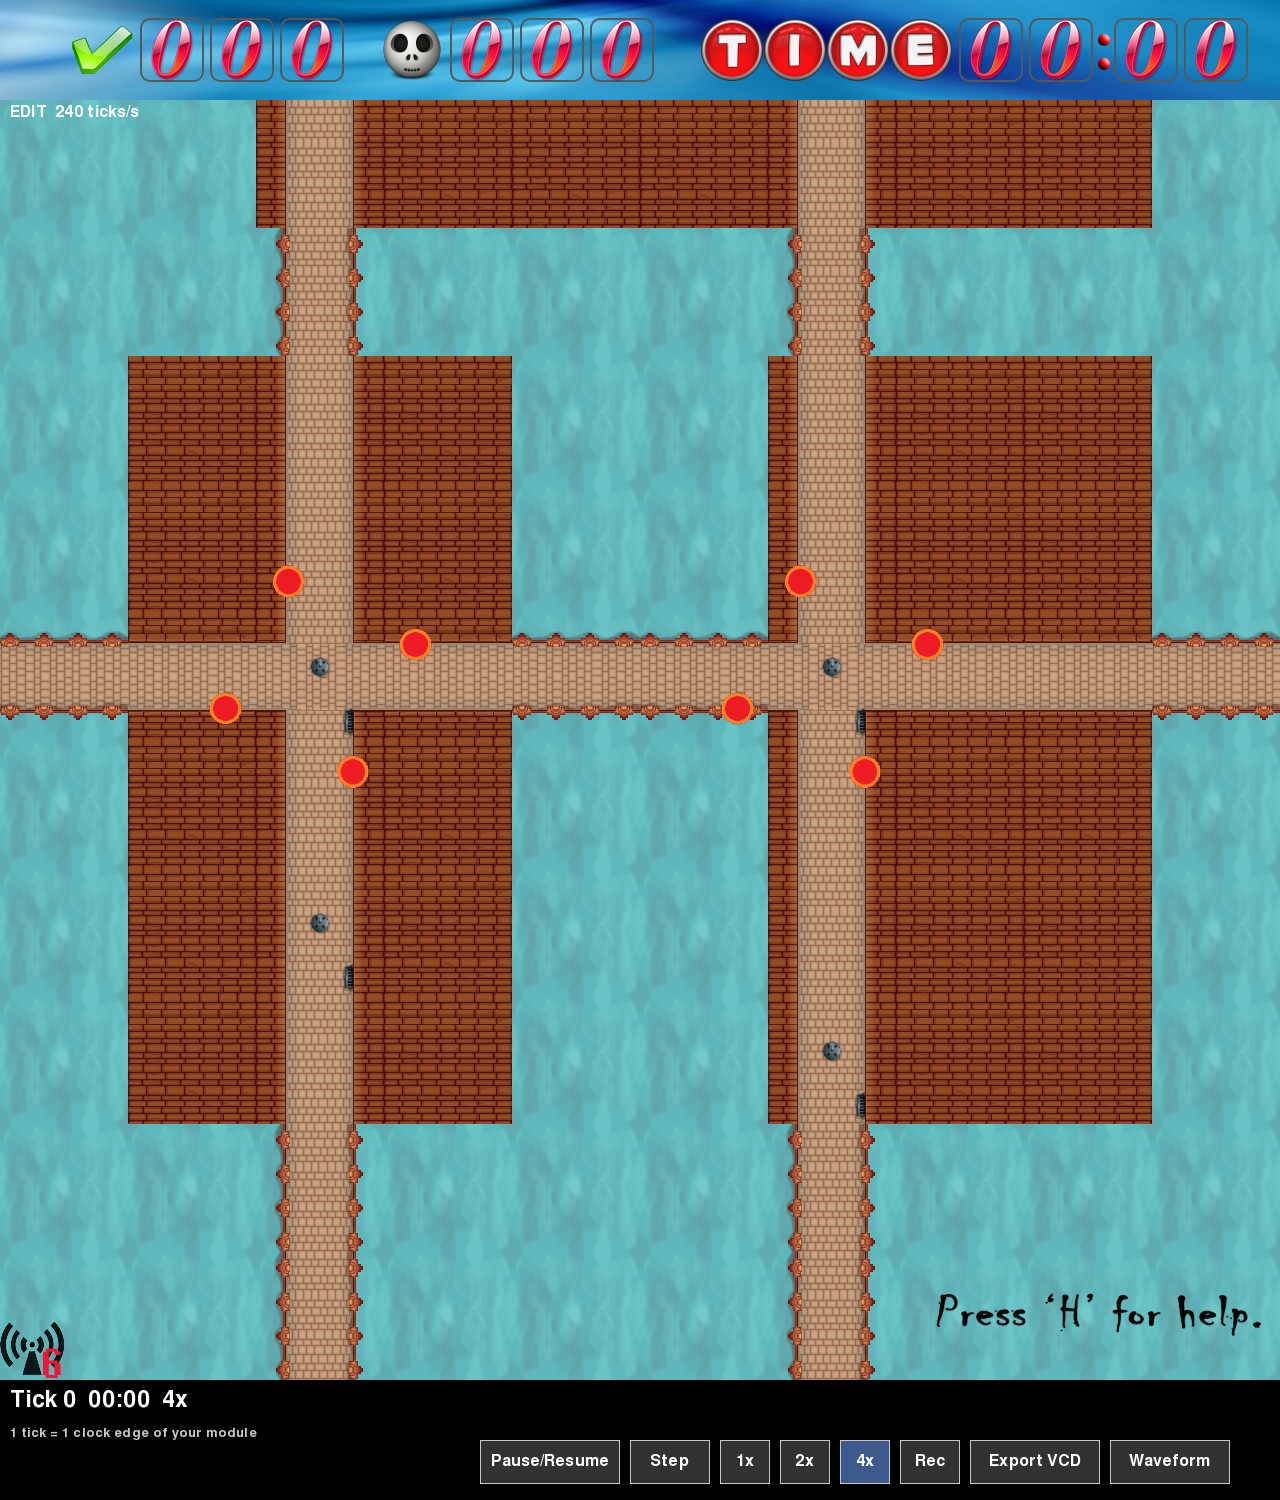
\includegraphics[width=0.46\linewidth]{images/mg-level-edit.png}
\caption{The main menu (left) and level 1 in the edit phase (right). The sensor pile with a ``6'' is at the
bottom-left of the map.}\label{fig:mg-menu}\label{fig:mg-level-edit}
\end{figure}

\subsection{Placing a sensor}

A level has seven general sensors, numbered 0 to 6. A sensor on a road tile tells your Verilog whether a car is
on that tile and where it is going. Sensors can only be placed before the start (the edit phase).

\begin{enumerate}
\item Click the sensor pile at the bottom-left of the map. The highest-numbered unplaced sensor follows the
mouse (Figure~\ref{fig:mg-sensor-in-hand}).
\item Click a road tile that is not part of an intersection. The sensor is placed and the sensor file is saved
(Figure~\ref{fig:mg-sensor-placed}). Click a placed sensor to pick it up again; right-click removes it; the key
\ui{C} removes all.
\end{enumerate}

\begin{figure}[H]\centering
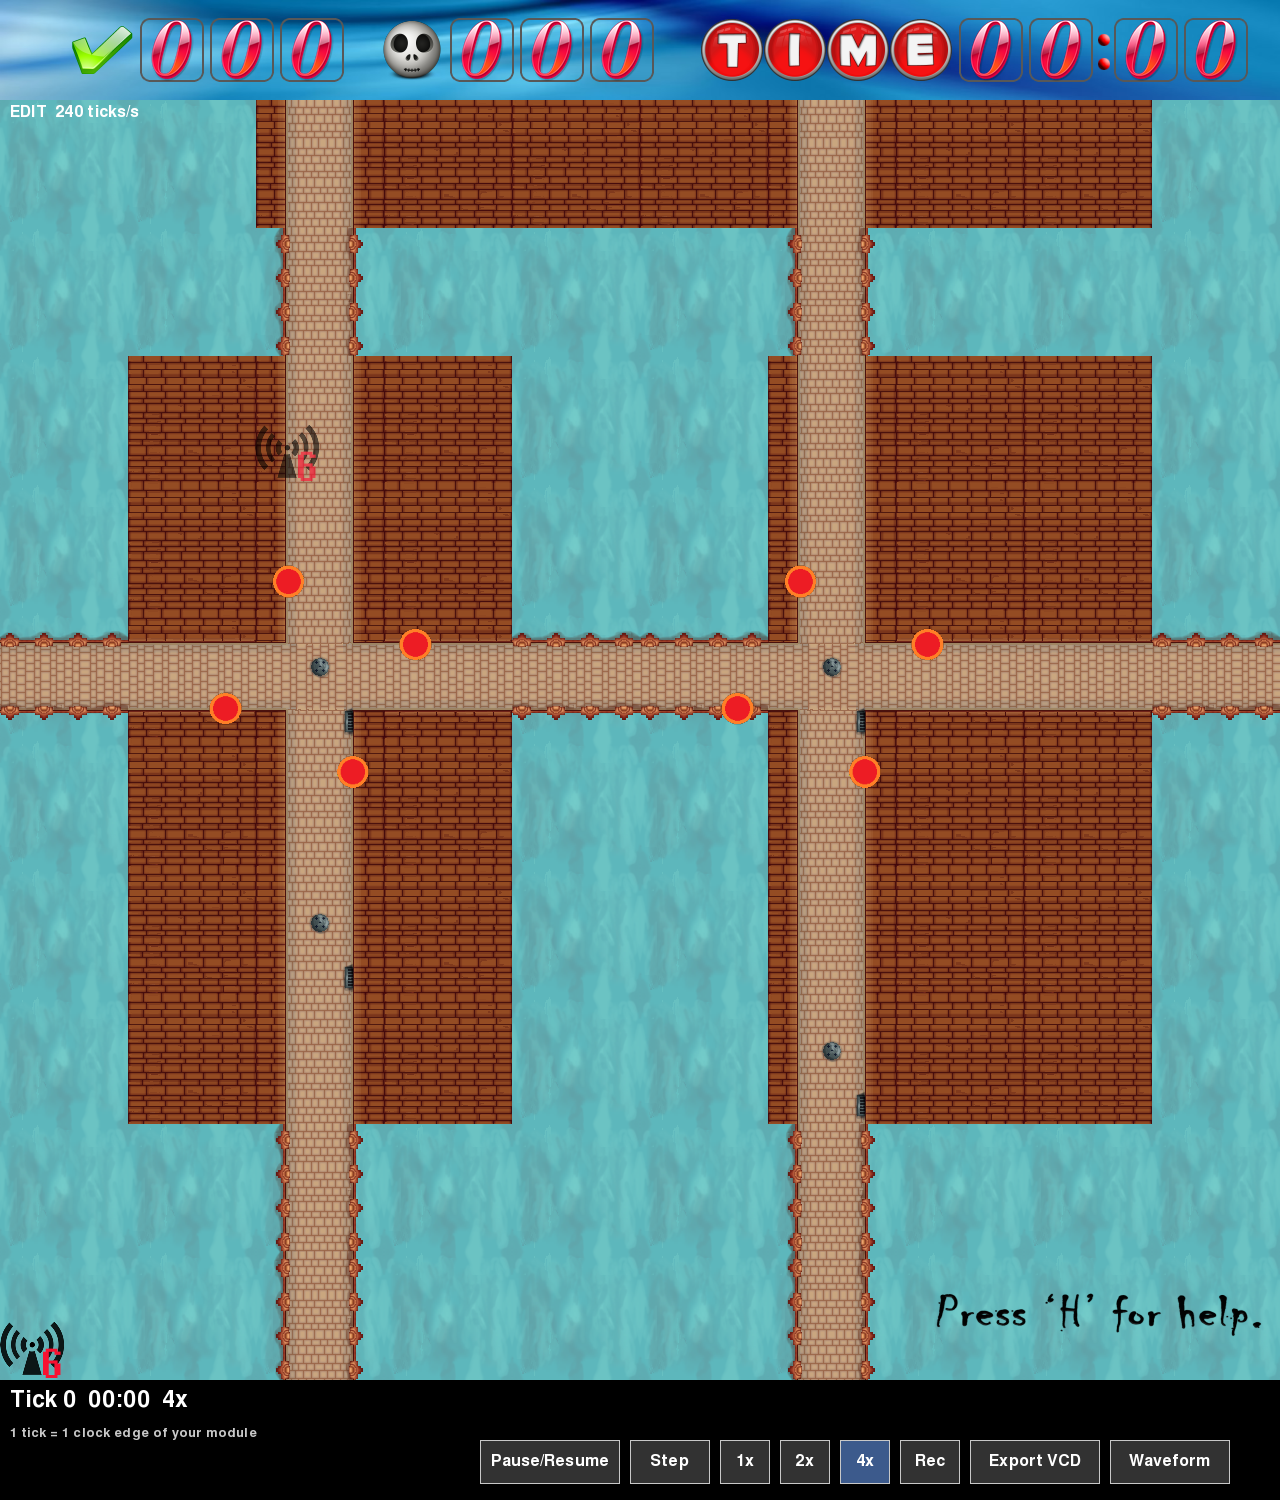
\includegraphics[width=0.46\linewidth]{images/mg-sensor-in-hand.png}\hfill
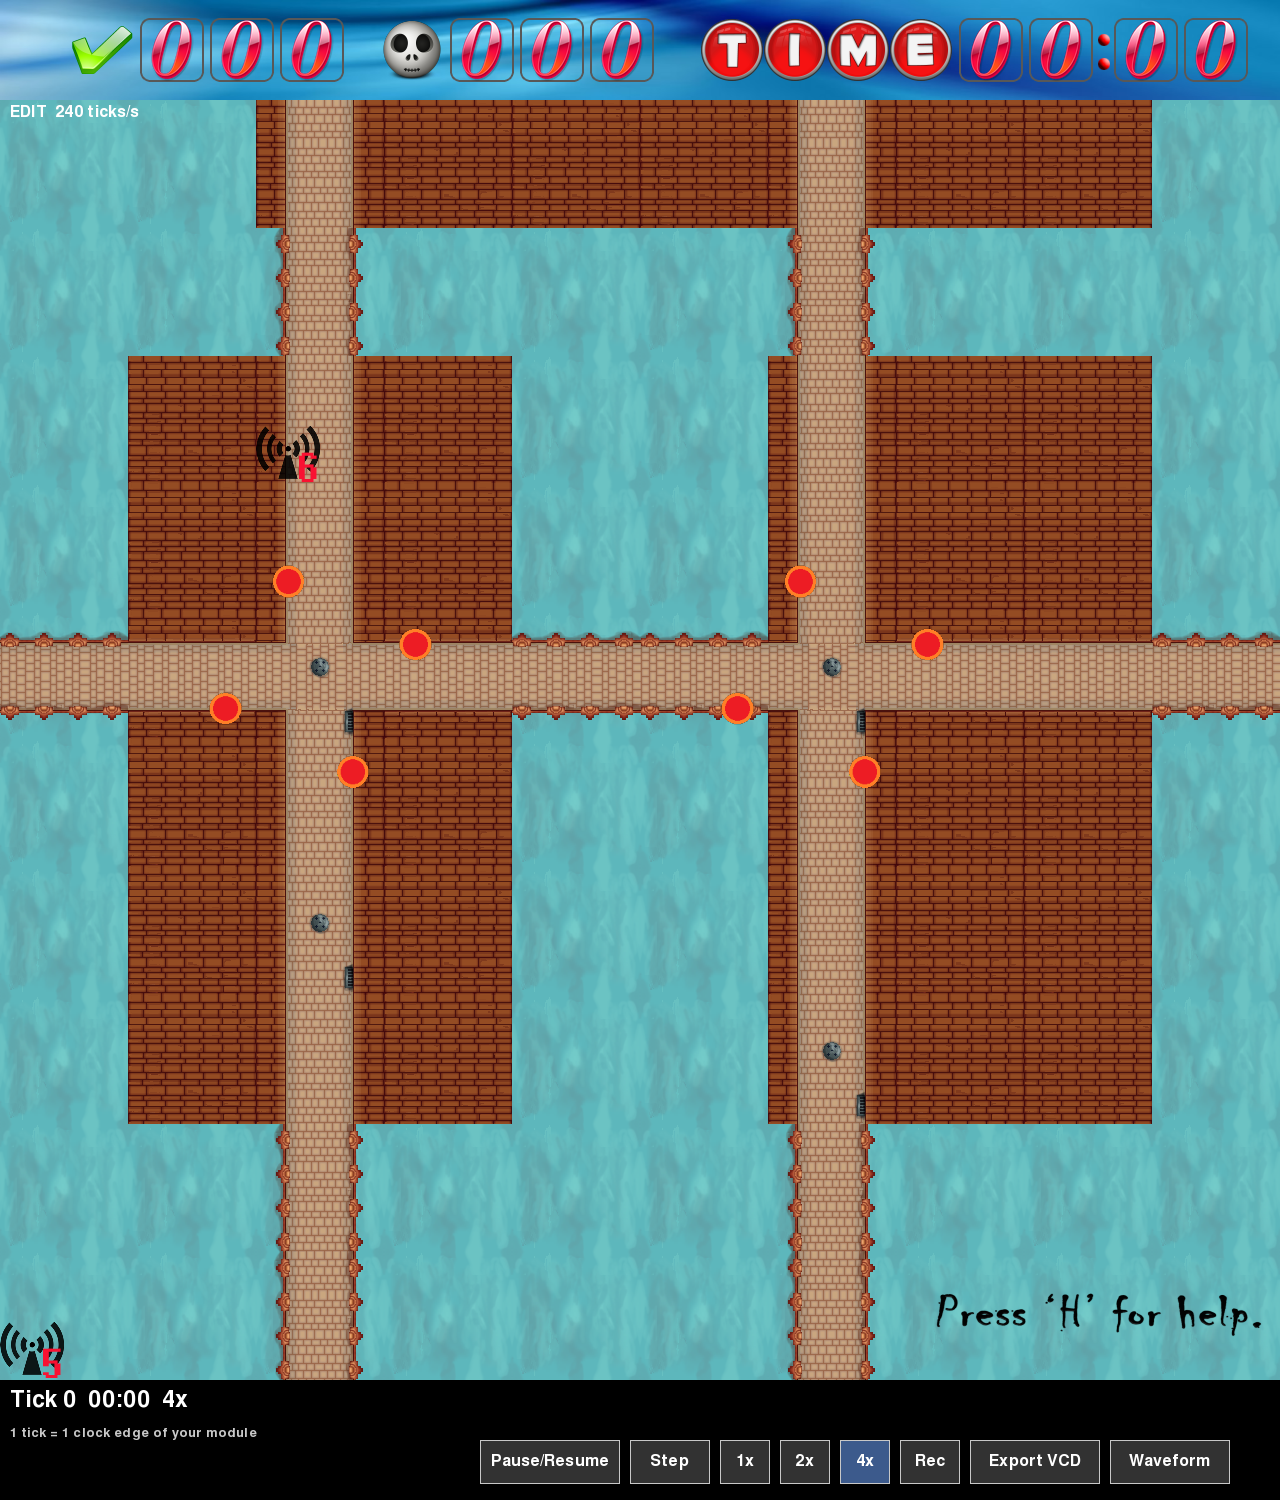
\includegraphics[width=0.46\linewidth]{images/mg-sensor-placed.png}
\caption{Sensor 6 in the hand, and placed on a road tile north of the first intersection.}\label{fig:mg-sensor-in-hand}\label{fig:mg-sensor-placed}
\end{figure}

\subsection{Editing the Verilog of a light}

\begin{enumerate}
\item Click an intersection. The Verilog editor window opens with the file of that light
(Figure~\ref{fig:ve-open}). The module \cmd{light1} has the ports \cmd{clk}, \cmd{rst} (active low),
\cmd{sensor\_light} (8 bits: the entries and the inside of this intersection), \cmd{general\_sensors} (30 bits: the
sensors you placed), the four outputs \cmd{outN}, \cmd{outS}, \cmd{outE}, \cmd{outW} (3 bits: 0 Stop, 1 Forward only,
2 Left only, 3 Right only, 4 Go) and an optional \cmd{debug\_port}.
\item For this tutorial we make one small change to the starter, so that the game shows us what the sensors
deliver: the line \cmd{assign debug\_port = sensor\_light;} becomes \cmd{assign debug\_port = general\_sensors;},
and a comment line is added at the top. The pictures below were made after this change.
\item Press \ui{Verify} (the green tick) to compile the file with Odin III (Figure~\ref{fig:ve-verified}).
\item Tick a box in the picture of the intersection, or type bits in the \ui{Internal Sensors} field, and press
\ui{Simulate} (the green triangle). The editor steps the module one clock cycle and prints the outputs; here a
car waits on the north entry (bit 6) and the light answers \cmd{OutN = 4}, Go (Figure~\ref{fig:ve-simulated}).
\end{enumerate}

\shot{ve-open}{The Verilog editor with the file of the first light (the starter with the change of step 2).}
\shot[0.9]{ve-verified}{After \ui{Verify}.}
\shot[0.9]{ve-simulated}{After \ui{Simulate} with a car on the north entry.}

\subsection{Running the level}

\begin{enumerate}
\item Close the editor and press \ui{S} to start. Cars drive; the status line shows the speed and the tick rate; the
buttons under the map change the speed, step and record.
\item Press \ui{P} to pause when a car is on your sensor. In the pause the strip under the map lists, for every intersection,
the inputs of the last tick and its four outputs (Figure~\ref{fig:mg-run-paused}). Here \cmd{general=0x0c000000}: sensor 6
(bits 27 to 24) reads 1100, a car is on its tile (bit 27) and the low bits of the ending counter of its destination are 100. Press \ui{S} to resume.
\item When all cars are done the score screen shows the cars that passed and the time in ticks (Figure~\ref{fig:mg-score}).
The ten best results of every level are kept.
\end{enumerate}

\begin{figure}[H]\centering
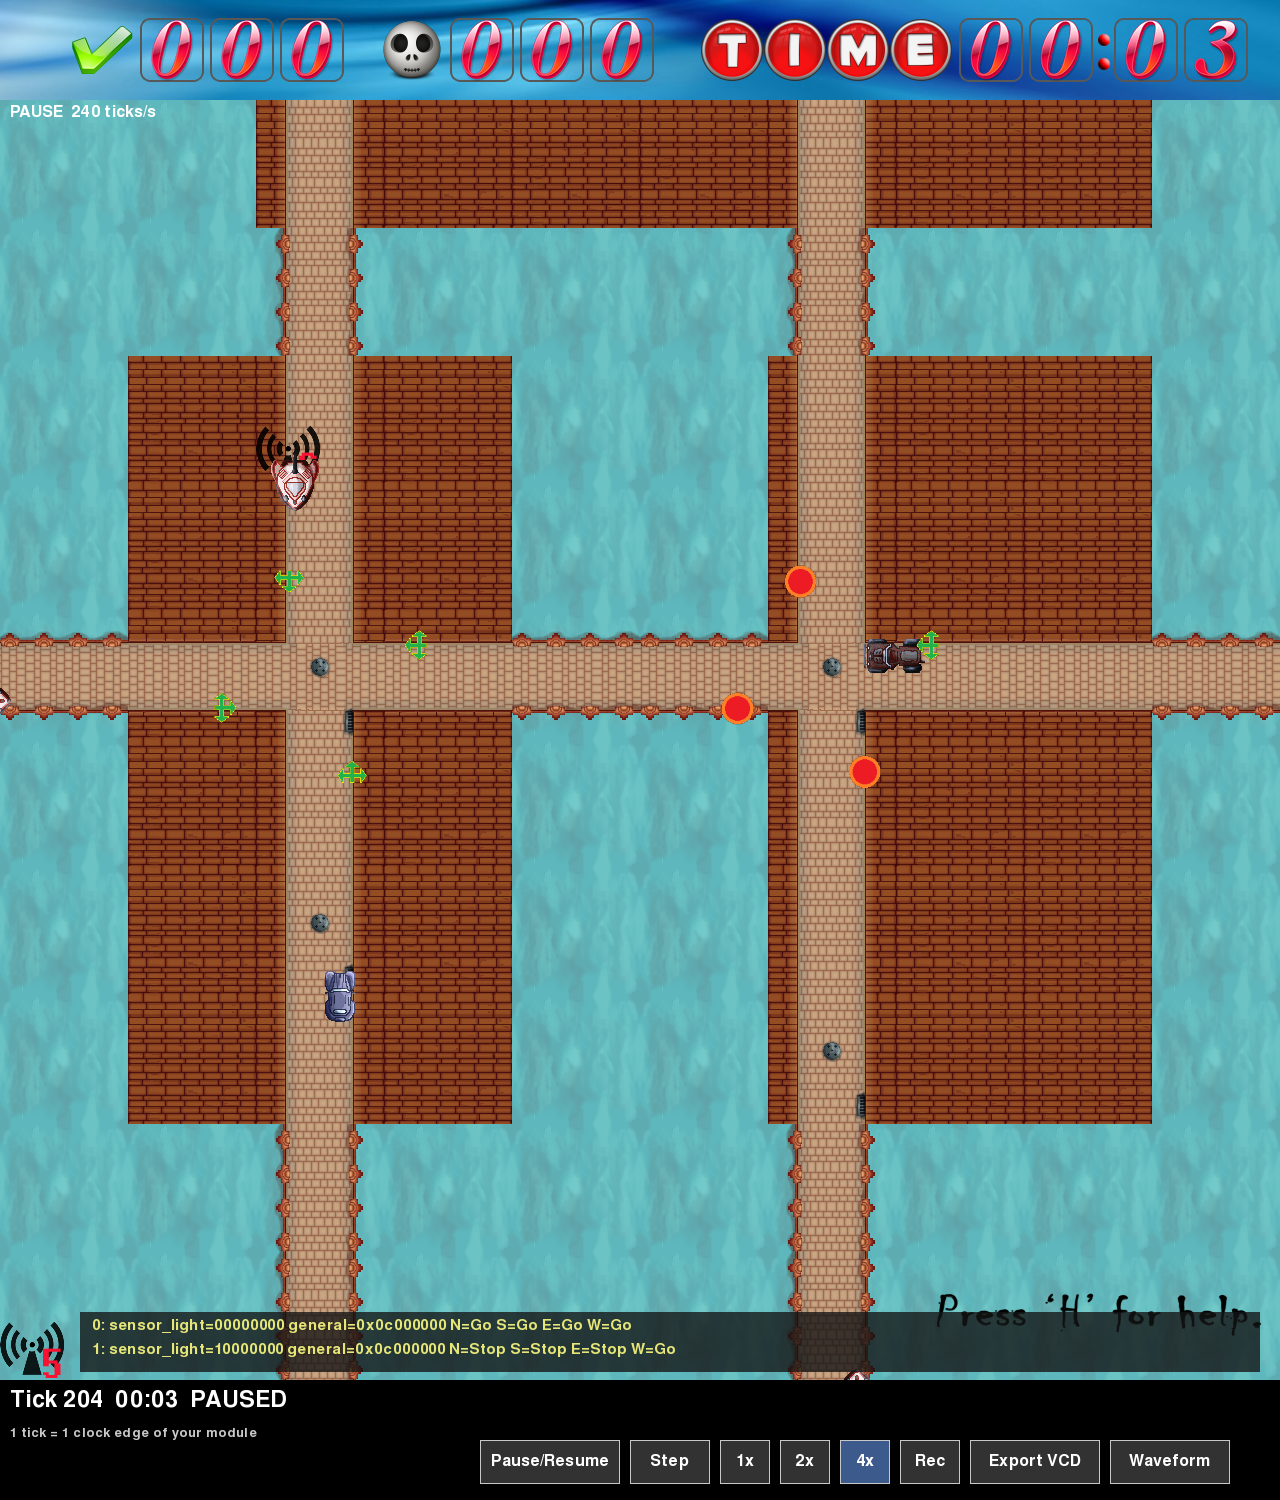
\includegraphics[width=0.62\linewidth]{images/mg-run-paused.png}
\caption{The level paused with a car on the sensor. The strip at the bottom shows the inputs and outputs of both
intersections.}\label{fig:mg-run-paused}
\end{figure}

\begin{figure}[H]\centering
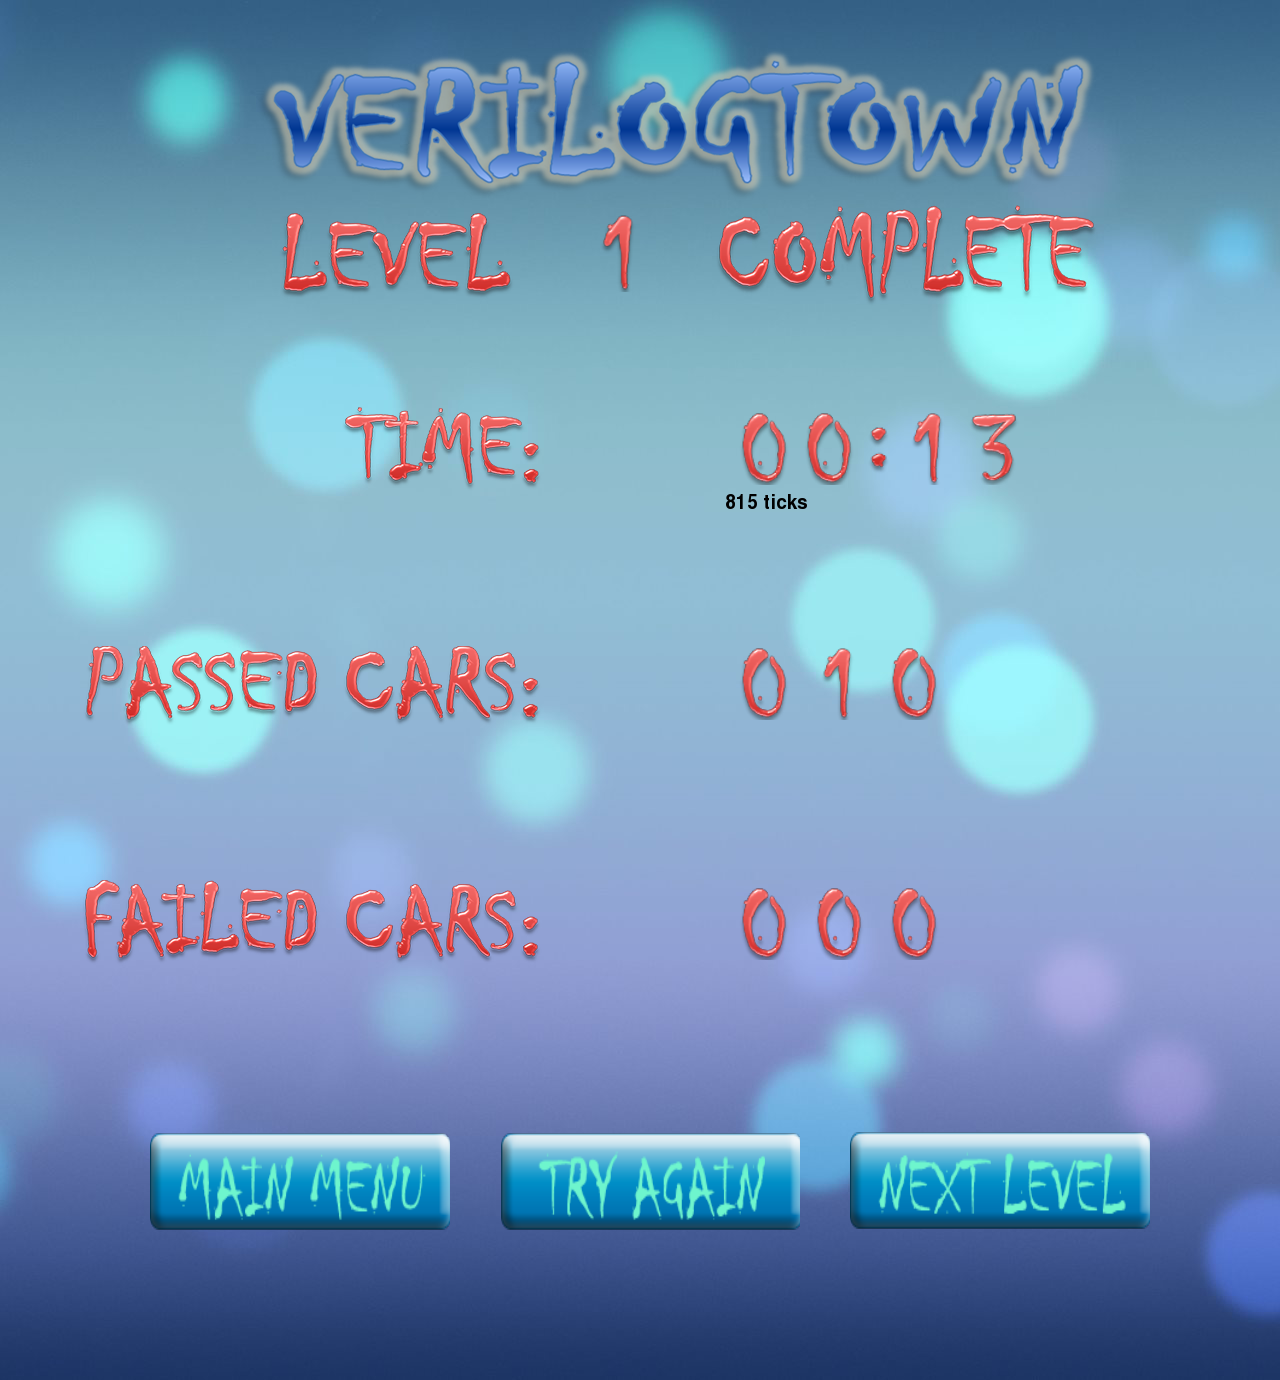
\includegraphics[width=0.62\linewidth]{images/mg-score.png}
\caption{The score screen of level 1.}\label{fig:mg-score}
\end{figure}

\subsection{The level editor}

You can make your own levels. Start \cmd{midgard-editor} (or \menu{Tools \gt Midgard III Level Editor}).
The start dialog (Figure~\ref{fig:le-start}) lets you create a level of a chosen even size or update an existing
level; Figure~\ref{fig:le-level1} shows level 1 loaded. You set the tile types, edit the cars with
\ui{Edit Cars} and \ui{Export} the level as the XML file and the map picture the game reads.

\begin{figure}[H]\centering
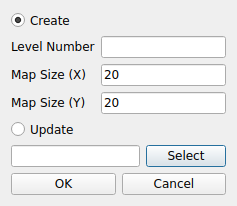
\includegraphics[width=0.40\linewidth]{images/le-start.png}\hfill
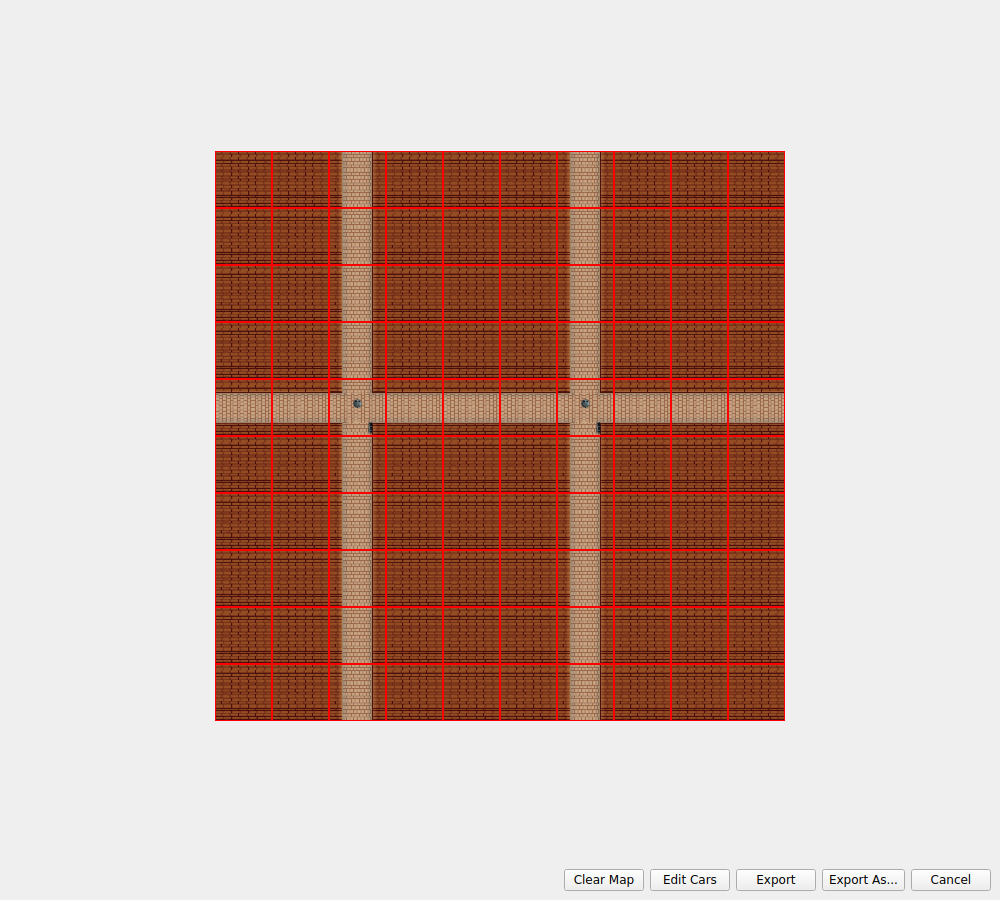
\includegraphics[width=0.54\linewidth]{images/le-level1.png}
\caption{The level editor: the start dialog (left) and level 1 loaded (right).}\label{fig:le-start}\label{fig:le-level1}
\end{figure}

\section{Where to Go Next}

\begin{itemize}
\item The user manual (\cmd{docs/user}, built with Sphinx) has one page for each part: getting started, projects,
running, the interface, simulation, Midgard III and the samples, with every command line flag and every key of
\cmd{wyrd.toml}.
\item The design documents are in \cmd{docs/specs}: the runner (W1), the interface (W2), Bifrost III (W3) and Midgard III (W4).
\item The Odin III manual explains the synthesis flow that the \cmd{odin3-flow} step runs.
\end{itemize}

\end{document}
